\title{Artificial Life - Project Proposal}
\author{Ryan Spangler}
\date{\today}

\documentclass[12pt]{article}

\usepackage{commath}
\usepackage{graphicx}
\usepackage{listings}
\usepackage{amsfonts}

% python highlighting ----------
\usepackage{color}
\usepackage{listings}
\usepackage{textcomp}
\usepackage{setspace}
%\usepackage{palatino}

\setcounter{secnumdepth}{0}

\begin{document}
\maketitle

\section{Introduction}

What is life?  The debate rages on.  Of the countless attempts at a definition, Rosen \cite{Rosen} chooses a completely different tactic that has no reference towards evolution, reproduction or the genetic code.  His claim is that an organism is defined by the entailment structure between its various components, specifically that all components of the organism are entailed by other components within the organism itself.  He calls this approach ``Relational Biology''.  

Specifically, the part of his discourse that is relevant to this project is that of the use of models in our understanding of physical phenomena.  The process of modeling is bringing into correspondence some real-world phenomena with a formal structure which can be analyzed and fabricated independently of the phenomena in question.  He claims that our models are only as rich as the entailment structure they provide.  The idea is that our traditional recursive modeling relation, coined by Newton and in heavy use to this day, has a paucity of entailment with which to model complex systems.  Rosen shows this relation as the following categorical diagram:

\begin{center}
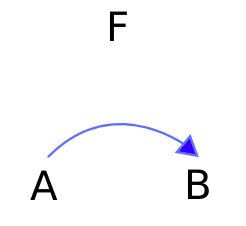
\includegraphics[scale=0.6]{newton.png}
\end{center}

The flaw in this diagram is that B is the only element that is entailed by anything.  Specifically, F itself is outside of all entailment, assumed to be part of the ``ambient'', a universal law translating A into B.  The elaboration he makes on this diagram provides a way for F to be entailed within the system, by invoking another component R which entails F from B and endowing B itself to be a function entailing R from F.  

\begin{center}
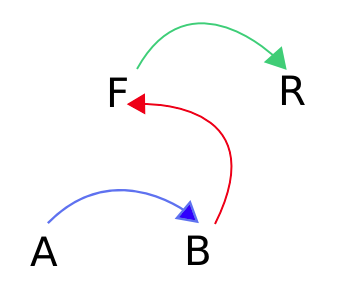
\includegraphics[scale=0.6]{rosen.png}
\end{center}

This is the diagram I am hoping to implement in some form over the course of this project.  

\section{Plan}

The plan is to implement this using javascript (for maximum dissemination) with the A component coming from user input, and F, B and R implemented as a dynamic executable tree composed of operations that work on and manipulate these same trees.  Though F, B and R represent different components of the system, in order to implement the diagram it seems that they should be of the same basic structure (much of this project is still conjecture).  The key is that whatever structure these elements are composed of must be able to operate on and be operated upon, to act as both program and data.  

There will be an interactive medium, a canvas where the interactions will take place and visual feedback will be given.  The trees can be displayed as they are modified by this circularly entailed process.  

I am not certain what the effect will be even, I will consider it a success if I am able to recreate the Rosen diagram in any form.  This is more of an experiment than a definitive product.  

\section{Logistical Concerns}

Though the diagram could be interpreted to mean that the functions F, B and R are replaced every time, I am interpreting it to mean that, for instance, B is a function which reads the tree F and uses this information to modify the tree R.  So in effect, there will be a pointer into F which is the currently read node, and a pointer into R which will be the currently modified node.  The program represented by the executable tree in B will be executed once each time step, which will basically be a branching conditional linking ``recognizers'', or conditions, to operations which act on the executable tree.  Parallel execution will be simulated in the traditional cellular automata manner, with all effects being calculated in one sweep and then applied in the next, so that every execution is reading a consistent state.  The operations themselves will have to be designed, with a tentative subset of tree operations being proposed: cutting, splicing adding and modifying nodes in the target tree.  There could also be operations that pertain to the visualization medium A.  

Another consideration is possibly applying a form of energy in the operations, in that an operation consumes a particular piece of data from A (the environment) in order to carry out its task.  It is not yet determined if this is necessary, but I suspect something like this will find its way into the design.

In the end, this could be used as a kind of discrete signal processor, with A being a signal from whatever application domain is desired and the tree F operating on A to modify B, B reading F to modify R and R reading from B to modify F, this entire process generating a dynamic form of behavior that embodies in executable form the diagram proposed by Rosen.  

Sounds like an adventure?  We will see what happens.

\bibliographystyle{plain}
\bibliography{proposal}

\end{document}  

